%\documentclass{article}
%\usepackage{graphicx,subfigure}
%\begin{document}

\begin{figure}[!h]
  \centering
   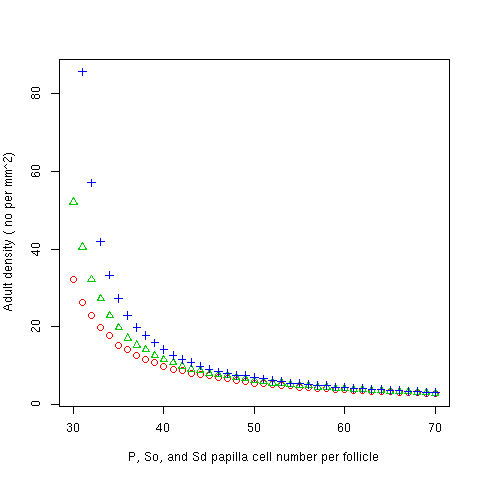
\includegraphics[width=0.9\textwidth]{avecellnodens.png}
  \caption{Calculated values of adult follicle density at a range of values of the parameters $C_{P}$ , $C_{So}$, and $C_{Sd}$,  from equations ~\ref{eqn:prim} to ~\ref{eqn:sd3} with values for the other 19  parameters fixed at the values given in Table~\ref{tab:base}. The three sets of points correspond to three values of the parameter $C_{b}$, red=.050, green=.052, blue=.054, the base value for this cell birth probability parameter being too high to use}
  \label{fig:avecellnodens}
\end{figure}

%\end{document}

